\documentclass[10pt]{article}
\usepackage{picinpar,graphicx,bm}
\usepackage[UTF8]{ctex}
\usepackage{booktabs}
\usepackage{diagbox}
\usepackage{subfigure}
\usepackage{float}
\usepackage{cases}
\usepackage{multirow}
\usepackage{booktabs}
\newcommand{\upcite}[1]{\textsuperscript{\textsuperscript{\cite{#1}}}}



\usepackage{bbding}
\usepackage{pifont}
\usepackage{wasysym}
\usepackage{amssymb}
\usepackage{threeparttable}


\usepackage{listings}
\usepackage{xcolor}
% 定义可能使用到的颜色
\definecolor{CPPLight}  {HTML} {686868}
\definecolor{CPPSteel}  {HTML} {888888}
\definecolor{CPPDark}   {HTML} {262626}
\definecolor{CPPBlue}   {HTML} {4172A3}
\definecolor{CPPGreen}  {HTML} {487818}
\definecolor{CPPBrown}  {HTML} {A07040}
\definecolor{CPPRed}    {HTML} {AD4D3A}
\definecolor{CPPViolet} {HTML} {7040A0}
\definecolor{CPPGray}  {HTML} {B8B8B8}
\lstset{
    columns=fixed,    
   % numbers=left,                                        % 在左侧显示行号
    frame=none,                                          % 不显示背景边框
    backgroundcolor=\color[RGB]{245,245,244},            % 设定背景颜色
    keywordstyle=\color[RGB]{40,40,255},                 % 设定关键字颜色
    numberstyle=\footnotesize\color{darkgray},           % 设定行号格式
    commentstyle=\it\color[RGB]{0,96,96},                % 设置代码注释的格式
    stringstyle=\rmfamily\slshape\color[RGB]{128,0,0},   % 设置字符串格式
    showstringspaces=false,                              % 不显示字符串中的空格
    language=c++,                                        % 设置语言
    morekeywords={alignas,continute,friend,register,true,alignof,decltype,goto,
    reinterpret_cast,try,asm,defult,if,return,typedef,auto,delete,inline,short,
    typeid,bool,do,int,signed,typename,break,double,long,sizeof,union,case,
    dynamic_cast,mutable,static,unsigned,catch,else,namespace,static_assert,using,
    char,enum,new,static_cast,virtual,char16_t,char32_t,explict,noexcept,struct,
    void,export,nullptr,switch,volatile,class,extern,operator,template,wchar_t,
    const,false,private,this,while,constexpr,float,protected,thread_local,
    const_cast,for,public,throw,std,size_t,__global__,__device__,__host__},
    emph={map,set,multimap,multiset,unordered_map,unordered_set,
    unordered_multiset,unordered_multimap,vector,string,list,deque,
    array,stack,forwared_list,iostream,memory,shared_ptr,unique_ptr,
    random,bitset,ostream,istream,cout,cin,endl,move,default_random_engine,
    uniform_int_distribution,iterator,algorithm,functional,bing,numeric,},
    emphstyle=\color{CPPViolet}, 
    frame=shadowbox,
    basicstyle=\footnotesize\ttfamily,
    tabsize=4,
}

\newcommand{\tabincell}[2]{\begin{tabular}{@{}#1@{}}#2\end{tabular}}  
% Keywords command
\providecommand{\keywords}[1]{\textbf{\textit{Keywords ---}} #1}



%layout
\usepackage{calc} 
\setlength\textwidth{7in} 
\setlength\textheight{9in} 
\setlength\oddsidemargin{(\paperwidth-\textwidth)/2 - 1in}
\setlength\topmargin{(\paperheight-\textheight -\headheight-\headsep-\footskip)/2 - 1.5in}


\title{Summary for Graph Theory}
\author{Linlin Ge}
\date{}
\CTEXoptions[today=old]
\begin{document}
\maketitle

\section{Common Graph}
\subsection{Gabriel Gragh (GG)}
It is the graph $G$ with vertex set $S$ in which any points are adjacent precisely if they are distinct.

\begin{figure}[htbp]
\begin{minipage}[t]{0.45\linewidth}
\centering
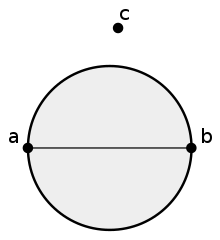
\includegraphics[scale=0.4]{pic/Gabriel_Pairs.png}
\caption{Gabriel Pairs}
\end{minipage}%
\begin{minipage}[t]{0.45\linewidth}
\centering
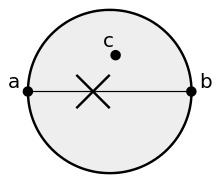
\includegraphics[scale=0.4]{pic/Not_Gabriel_Pairs.png}
\caption{Not Gabriel Pairs}
\end{minipage}

\end{figure}


\subsection{Relative Neighborhood Graph (RNG)}
The relative neighborhood graph (RNG) is an undirected graph defined on a set of points in the Euclidean plane by connecting two points p and q by an edge whenever there does not exist a third point r that is closer to both p and q than they are to each other.

\subsection{Urquhart graph}
The graph formed by removing the longest edge from every triangle in the Delaunay triangulation, was originally proposed as a fast method to compute the relative neighborhood graph. Although the Urquhart graph sometimes differs from the relative neighborhood graph it can be used as an approximation to the relative neighborhood graph.

\begin{thebibliography}{1}



\end{thebibliography}



\end{document}
